\section[Drude Theory of Electrons in Metals Sommerfeld Free Electron Theory of Electrons in Metals]{\hyperlink{toc}{Drude Theory of Electrons in Metals Sommerfeld Free Electron Theory of Electrons in Metals}}


\subsection*{3.1 \quad Drude Theory of Transport in Metals}

\begin{enumerate}[label=(\alph*)]
\item Assume a scattering time $\tau$ and use Drude theory to derive an expression for the conductivity of a metal.


\divider 

\begin{itemize}
    \item This is the same derivation from class, so let's consider the derived equation of motion from the Drude model when we have a non-zero electrical field (with $\mathbf{B}$ still 0):
    
    \[ \vec{E} \neq 0, \quad \vec{B} = 0 \]

    Equation of motion:

    \[ \dv{\vec{p}}{t} = -e \vec{E} - \frac{\vec{p}(t)}{\tau} \]

    \item We can now define the conductivity of a metal, $\sigma$, which is the constant of proportionality between the current density $\vec{j}$, and the applied electric field $\vec{E}$.
    
    \begin{center}
        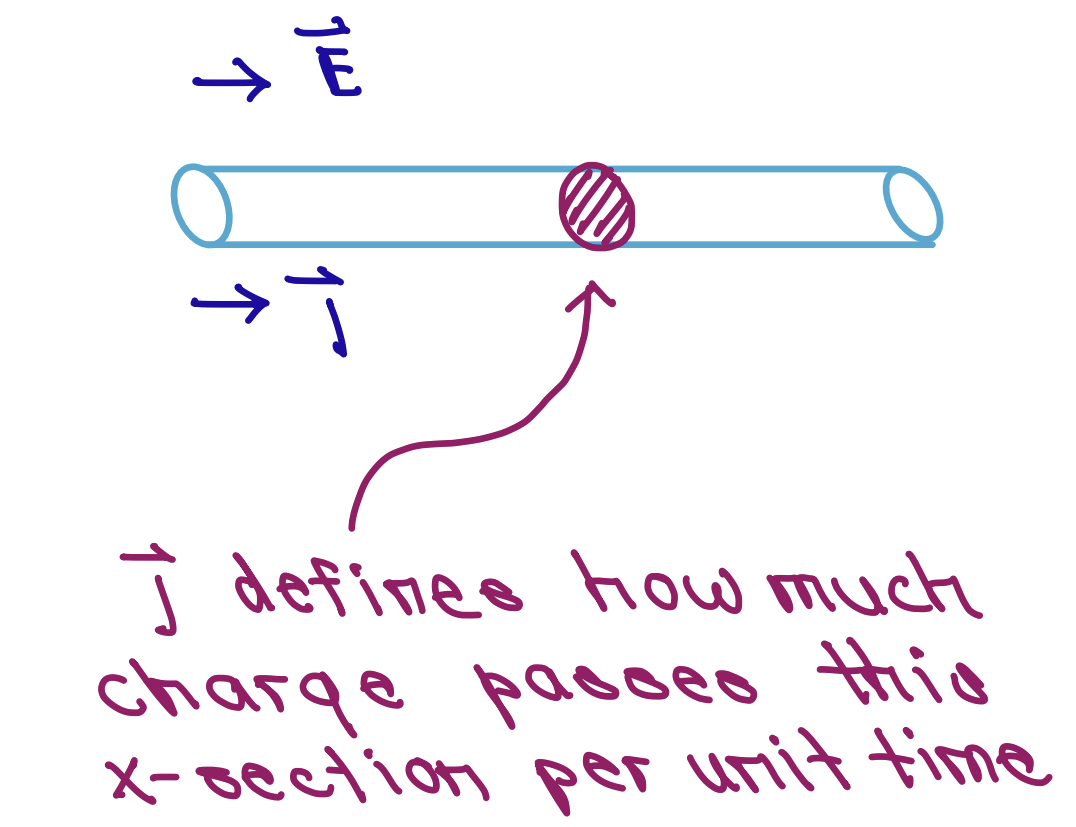
\includegraphics[width = 0.3 \linewidth]{Images/current-density.png}
    \end{center}

    where

    \[\vec{j} = \text{current density} \]
    
    which is the charge per unit time per unit area

    \[ \vec{j} = - n e \vec{v} \]

    where $n$ is the density of electrons   

    \[ \brackets*{e^-/m^3}\brackets*{C/e^-} \brackets*{m/s} = \frac{C}{m^2 \cdot s} \]

    \[ \vec{j} = \frac{e^2 n \tau}{m} \vec{E} \Rightarrow \boxed{\sigma = \frac{e^2 n \tau}{m}} \text{ units } \brackets*{\Omega^{-1} m^{-1}}\]

\end{itemize}


\item Define the resistivity matrix $\underset{\sim}{\rho}$ as 
$\mathbf{E} = \underset{\sim}{\rho}\,\mathbf{j}$. 
Use Drude theory to derive an expression for the matrix 
$\underset{\sim}{\rho}$ for a metal in a magnetic field. 
(You may assume $\mathbf{B}$ parallel to the $\hat{z}$ axis. 
The under-tilde means that the quantity $\rho$ is a matrix.) 
Invert this matrix to obtain an expression for the conductivity matrix 
$\underset{\sim}{\sigma}$.

\divider

\begin{center}
    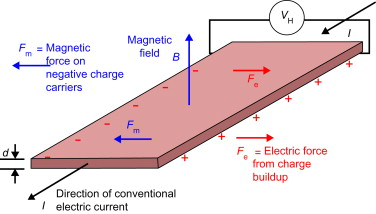
\includegraphics[width = 0.4 \linewidth]{Images/hall-effect.jpg}
\end{center}

For simplicity of typsetting I will use $\rho$ instead of $\underset{\sim}{\rho}$ (and likewise for $sigma$) until the final step.

Recall -- equation of motion derived in lecture 5:

\[ \dv{\vec{p}}{t} = F - \frac{\vec{p}(t)}{\tau} \]

\[ \dv{\vec{p}}{t} = -e \left( \vec{E} + \vec{v} \times \vec{B} \right) - \frac{\vec{p}(t)}{\tau} \]

If we again assume steady state ($\dv{p}{t} = 0$), we get:

\[ 0 = -e \left( \vec{E} + \vec{v} \times \vec{B} \right) - \frac{\vec{p}(t)}{\tau} \]

\[ e \vec{E} = - e \left( \vec{v} \times \vec{B} \right) - \frac{\vec{p}(t)}{\tau}\]

\[ \vec{E} = - \left( \vec{v} \times \vec{B} \right) - \frac{\vec{p}(t)}{e \tau}\]

Recall that $\vec{j} = -ne \vec{v}$ and $\vec{p} = m \vec{v}$. Thus, we can substitute these into the equation as $\vec{p} = \frac{m}{-ne} \vec{j}$ and $\vec{v} = \frac{-1}{ne} \vec{j}$:

\[ \vec{E} = \left( \frac{m}{ne^2 \tau} \right) \vec{j} + \left( \frac{1}{ne} \right) \vec{j} \times \vec{B} \]

where the first term is "longitudinal"  and the second term is off diagonal. Here $\vec{B} = B_z \hat{z}$. We are given the quation:
\[ \vec{B} \parallel \hat{z}, \quad \vec{j} \text{ can be applied along } \hat{x}, \hat{y}, or \hat{z} \]
    
\[ \mathbf{E} = \rho \mathbf{j} \]

We can define a 3 x 3 resistivity matrix for $\undertilde{\rho}$.

\[ \vec{E} = \left( \frac{m}{ne^2 \tau} \right) \begin{pmatrix}
    j_x \\ j_y \\ j_z
\end{pmatrix} + \left(\frac{1}{ne} \right) \begin{pmatrix}
    j_x , j_y , j_z
\end{pmatrix} \times \begin{pmatrix}
    0 \\ 0 \\ B_z
\end{pmatrix} \]

Look at just the cross product we can use the determinant form:

\[ \begin{vmatrix}
    \hat{x} & \hat{y} & \hat{z} \\
    j_x & j_y & j_z \\
    0 & 0 & B_z
\end{vmatrix}  =  j_y B_z \hat{x} - j_x B_z \hat{y} \]


Giving us
\[ \vec{E} = \begin{pmatrix}
\left( \frac{m}{ne^2 \tau} \right) j_x + \left(\frac{B_z}{ne} \right) j_y \\
\left( \frac{m}{ne^2 \tau} \right) j_y - \left(\frac{B_z}{ne} \right) j_x \\
\left( \frac{m}{ne^2 \tau} \right) j_z
\end{pmatrix} \]

Issolating the $\vec{j}$ we can pull out the $\rho$ term.

\[ \vec{E} = \begin{pmatrix}
    \frac{m}{ne^2\tau}& \frac{B}{ne}& 0 \\
    -\frac{B}{ne}&\frac{m}{ne^2\tau}& 0 \\
    0& 0& \frac{m}{ne^2\tau}\\
\end{pmatrix}
\begin{pmatrix}
    j_x \\ j_y \\ j_z
\end{pmatrix}\]

\[ \underset{\sim}{\rho} = \begin{pmatrix}
    \rho_{xx} & \rho_{xy} & 0 \\
    \rho_{yx} & \rho_{yy} & 0 \\
    0 & 0 & \rho_{zz}
    \end{pmatrix} = \begin{pmatrix}
        \frac{m}{ne^2 \tau} & \frac{B}{ne} & 0 \\
        -\frac{B}{ne} & \frac{m}{ne^2 \tau} & 0 \\
        0 & 0 & \frac{m}{ne^2 \tau}
    \end{pmatrix}
 \]

\[ \rho_{xx} = \rho_{yy} = \rho_{zz} = \frac{m}{ne^2 \tau} \]

Hall resistivity:

\[ \boxed{\rho_{xy} = -\rho_{yx} = \frac{B}{ne} }\]

We find that the application of a $\mathbf{B}$ field deflects the electrons causing a measurable potential difference in the orthogonal direction -- this is the Hall effect.

Now taking the inverse of the resistivity we can find the conductivity matrix. Since we have terms along the diagonal, we can split up the problem into a 2x2 inverse and a single element.

\[ A = \begin{pmatrix}
    \rho_{xx} & \rho_{xy} \\ -\rho_{xy} & \rho_{yy}
\end{pmatrix} \]

\[ \det(A) = \rho_{xx} \rho_{yy} + \rho_{xy}^2 \]

\[ A^{-1} = \frac{1}{\det(A)} \begin{bmatrix}
    d & -b \\ -c & a
\end{bmatrix} = \frac{1}{\rho_{xx} \rho_{yy} + \rho_{xy}^2} \begin{bmatrix}
    \rho_{yy} & -\rho_{xy} \\ \rho_{xy} & \rho_{xx}
\end{bmatrix}\]

\[ d = \rho_{zz} \Rightarrow d^{-1} = \rho_{zz}^{-1}\]

Thus, we can write the conductivity matrix as:

\[ \sigma = \rho^{-1} = \begin{pmatrix}
    A^{-1} & 0 \\ 0 & d^{-1}
\end{pmatrix} \]

\[ \sigma = \begin{pmatrix}
    \frac{\rho_{yy}}{\rho_{xx} \rho_{yy} + \rho_{xy}^2} & -\frac{\rho_{xy}}{\rho_{xx} \rho_{yy} + \rho_{xy}^2} & 0 \\ \frac{\rho_{xy}}{\rho_{xx} \rho_{yy} + \rho_{xy}^2} & \frac{\rho_{xx}}{\rho_{xx}\rho_{yy}+\rho_{xy}^2} & 0 \\ 0 & 0 & \frac{1}{\rho_{zz}}
\end{pmatrix} \]

Putting the terms for rho back in:

\[
\sigma = \begin{pmatrix}
    \dfrac{\frac{m}{ne^2\tau}}{\left(\frac{m}{ne^2\tau}\right)^2 + \left(\frac{B}{ne}\right)^2} & -\dfrac{\frac{B}{ne}}{\left(\frac{m}{ne^2\tau}\right)^2 + \left(\frac{B}{ne}\right)^2} & 0 \\
    \dfrac{\frac{B}{ne}}{\left(\frac{m}{ne^2\tau}\right)^2 + \left(\frac{B}{ne}\right)^2} & \dfrac{\frac{m}{ne^2\tau}}{\left(\frac{m}{ne^2\tau}\right)^2 + \left(\frac{B}{ne}\right)^2} & 0 \\
    0 & 0 & \dfrac{ne^2\tau}{m}
\end{pmatrix}
\]



\item Define the Hall coefficient.

    
\[ R_H = \frac{-\rho_{xy}}{|B|} = \frac{-1}{ne} \quad \text{ units } \brackets*{m^3/C}\]

    note: "normal" meteals have a negative $R_H$ (NOT a resistance).

    \begin{center}
        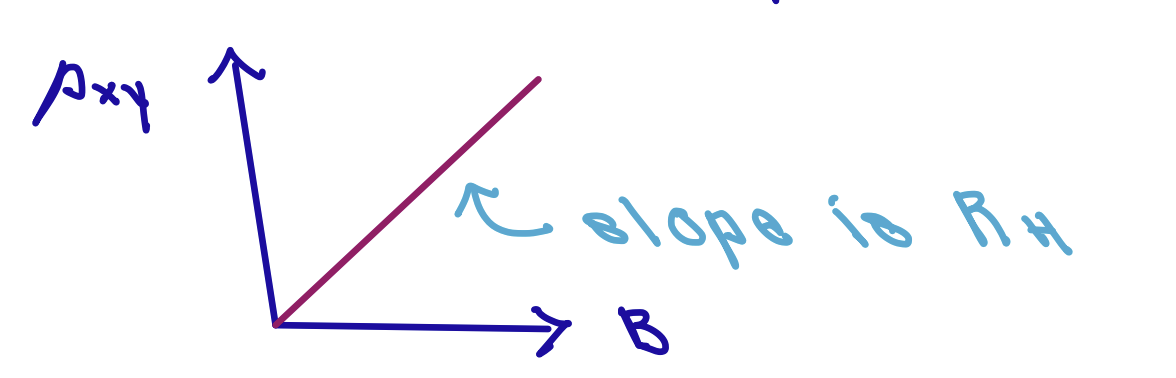
\includegraphics[width = 0.4 \linewidth]{Images/hall-effect-slope.png}
    \end{center}

Some metals have a positive Hall coefficient -- seeming to imply the existence of a positively charged carrier of electrical current. This is forshadowing for later in the course when we will get introduced to the concept of holes in semiconductors.

The Hall coefficient $R_H$ for copper (good metal) is of order 0.1 $mm^3/C$ and its resistivity at RT is of order $10^{-8} \Omega m$. The order of magnitude of the scattering time, $\tau$.
    
    \[ R_H = 0.1 mm^3/C = 10^{-10} m^3/C = \frac{-1}{n e} \]

    \[ \rho = \frac{1}{\sigma} = 10^{-8} \Omega m = \frac{m}{n e^2 \tau} \]

    \[ \tau = \frac{-m R_H}{e^2 \rho} = \frac{-\paren*{10^{-30}\, \text{kg}} \paren*{10^{-10} m^{3}/C}}{\paren*{-10^{-19} C} \paren*{10^{-8} \Omega m}} = 10^{-13} s \]

Average metal $\approx$ 10$^{-14}$ s, so this is reasonable. Scattering time is extraordinarile short. 


\item What properties of metals does Drude theory not explain well?

\item Consider now an applied AC field $\mathbf{E} \sim e^{i \omega t}$ which induces an AC current $\mathbf{j} \sim e^{i \omega t}$. Modify the above calculation (in the presence of a magnetic field) to obtain an expression for the complex AC conductivity matrix $\sigma(\omega)$. For simplicity in this case you may assume that the metal is very clean, meaning that $\tau \to \infty$, and you may assume that $\mathbf{E} \perp \mathbf{B}$. You might again find it convenient to assume $\mathbf{B}$ parallel to the $\hat{z}$ axis. (This exercise might look hard, but if you think about it for a bit, it isn’t really much harder than what you did above!)

\begin{itemize}
    \item At what frequency is there a divergence in the conductivity? What does this divergence mean? (When $\tau$ is finite, the divergence is cut off.)
    \item Explain how could one use this divergence (known as the cyclotron resonance) to measure the mass of the electron. (In fact, in real metals, the measured mass of the electron is generally not equal to the well-known value $m_e = 9.1095 \times 10^{-31}\,\mathrm{kg}$. This is a result of \textit{band structure} in metals, which we will explain in Part VI.)
\end{itemize}

\end{enumerate}
